\documentclass{article}
\usepackage{amsmath}
\usepackage{float}
\usepackage{fullpage}
\usepackage{parskip}
\usepackage{graphicx}
\usepackage{listings}
\usepackage{minted}

\usemintedstyle{tango}

\lstset
{
    basicstyle = \fontfamily{cmr},
    breaklines = true,
    breakindent = 0pt,
    mathescape
}
\title{Ph20 Assignment 3 (Part 2)}
\author{Ung Shu Fay}

\begin{document}
\maketitle

\section{Phase Space Trajectories}
    \begin{figure}[h!]
        \centering
        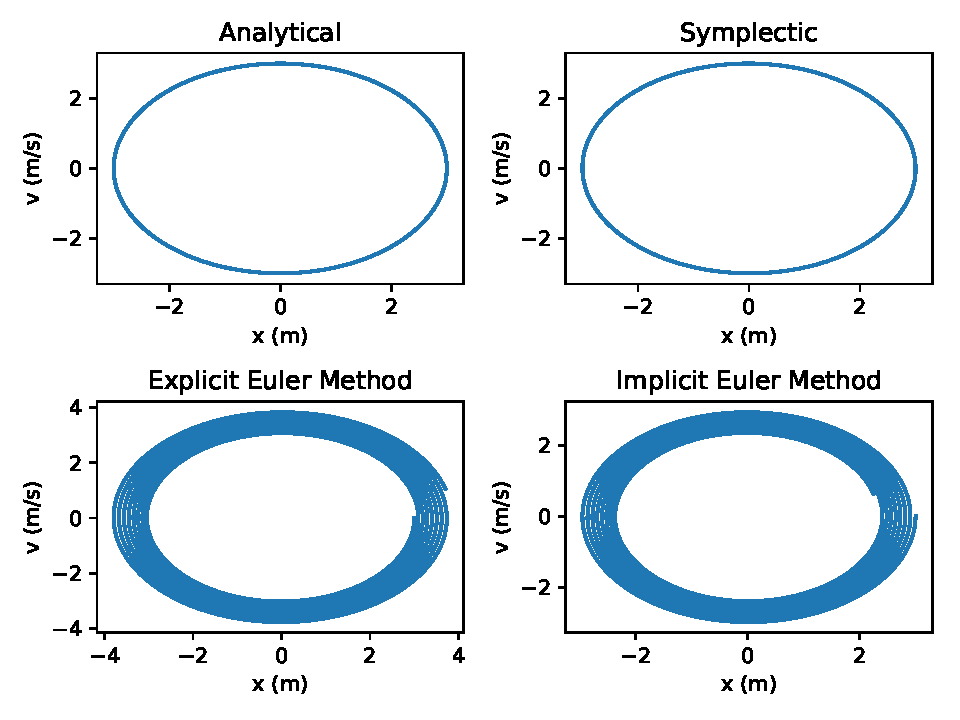
\includegraphics[scale=0.8]{phase_space.pdf}
        \label{phase}
    \end{figure}

    \lstinputlisting{phase_space.txt}

\section{Energy}
    \begin{figure}[h!]
        \centering
        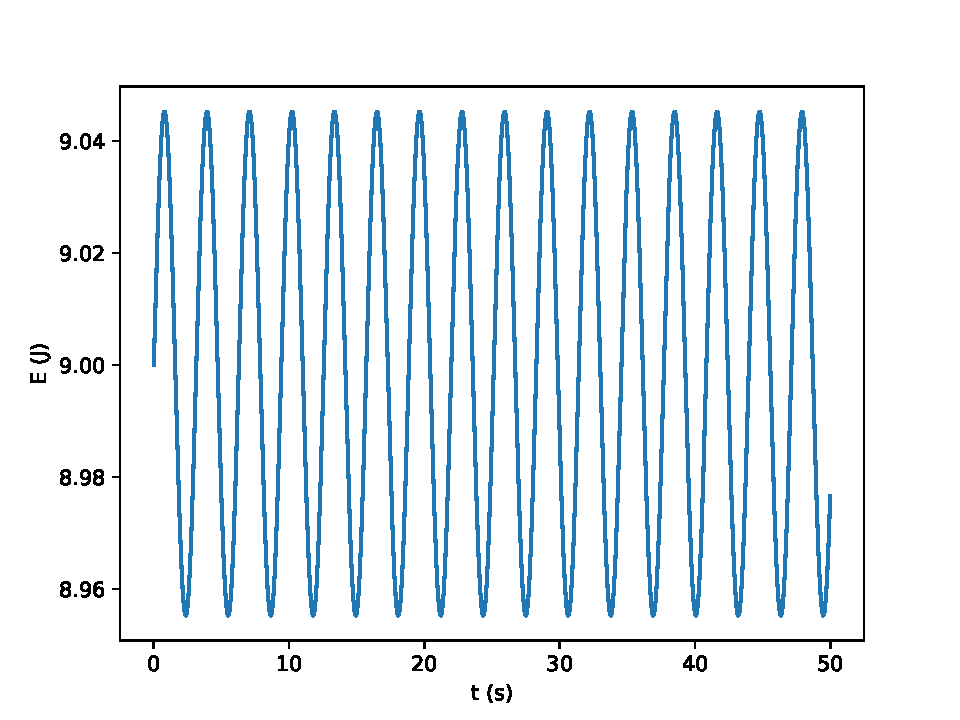
\includegraphics[scale=0.6]{energy.pdf}
        \label{energy}
    \end{figure}
    
    \lstinputlisting{energy.txt}

\section{Global Error}
    \begin{figure}[h!]
        \centering
        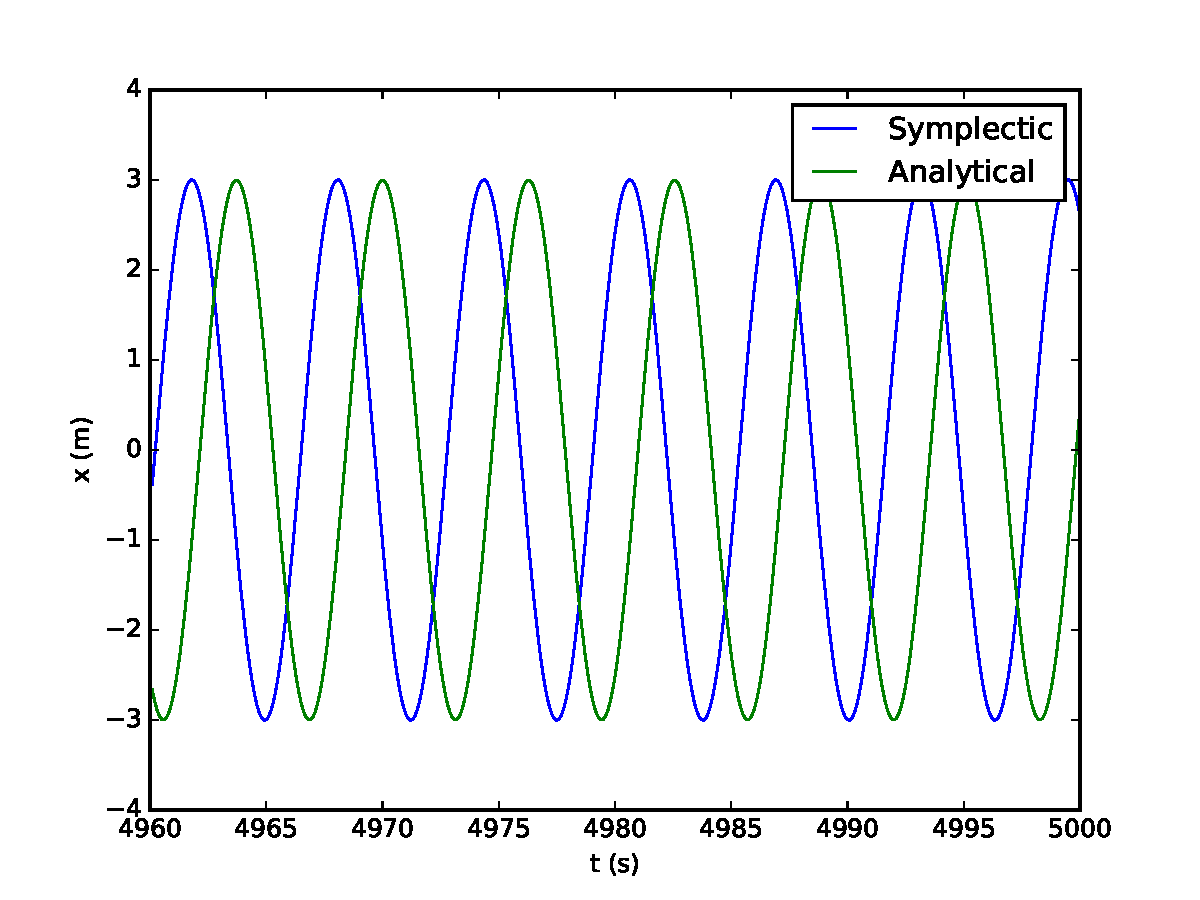
\includegraphics[scale=0.6]{error.pdf}	
        \label{error}
    \end{figure}
        
    \lstinputlisting{error.txt}

\break
\section{Makefile}
	\inputminted{make}{Makefile}

\section{Source Code}
	\inputminted{python}{phase.py}

\section{Git Log}
    \lstinputlisting[basicstyle = \ttfamily]{git.txt}

\end{document}
